\section{Annexe}

\subsection{Glossaire}

\noindent \textbf{GPIO} : \emph{General Purpose Input/Output}. Les ports GPIO sont des ports d'entrées-sorties très utilisés dans le monde des microcontrôleurs, en particulier dans le domaine de l'électronique embarquée, qui ont fait leur apparition au début des années 1980. Elles sont placées sur un circuit électronique afin de communiquer avec des composants électroniques et circuits externes. Il peut s'agir de détecteurs ou senseurs pour capter des données, ou encore de contrôler des commandes.

\noindent \textbf{IHM} : \emph{Interface Homme-Machine}. C'est l'interface qui permet à l' utilisateur de communiquer avec un ordinateur, une application ou un dispositif électronique(ici un le robot suiveur de ligne). L'IHM peut prendre différentes formes, telles que des écrans graphiques, des boutons, des claviers, des écrans tactiles, des commandes vocales, etc. Le but de l'IHM est de rendre la communication avec la technologie plus intuitive et plus accessible pour les utilisateurs.



\hfill Source : Wikipédia

\subsection{Documentation}

\noindent Les liens suivants sont destinées à la documentation techniques des composants principaux de notre robot suiveur de ligne.

Sommaire :
\begin{itemize}
    \item \href{https://www.nxp.com/docs/en/data-sheet/KL25P80M48SF0.pdf}{NXP FRDM KL25Z based on Arm® Cortex®-M0+ Core}
    \item \href{https://www.st.com/resource/en/datasheet/l298.pdf}{Double Pont en H L298}
    \item \href{https://www.st.com/resource/en/datasheet/l78l.pdf}{Régulateur 5V -> 3,3V L78L}
    \item \href{https://docs.rs-online.com/8525/0900766b816ed3dd.pdf}{Régulateur 12V -> 5V TSR 1-2450}
    \item \href{https://www.mouser.fr/datasheet/2/308/1/HCPL2631_D-1522483.pdf}{Optocoupleur HCPL2631}
    \item \href{https://www.mouser.fr/datasheet/2/239/LTV_8X6_series-2887056.pdf}{Optocoupleur LTV-816}
    \item \href{https://www.ti.com/lit/gpn/lm111-n}{Comparateur de tension LM111}
\end{itemize}

\subsection{Autres}

\vfill
\noindent\makebox[\linewidth]{\rule{.8\paperwidth}{.6pt}}\\[0.2cm]
I.U.T. Nice Côte d'Azur - SAE Robot - 2023 \hfill goofyBot
\noindent\makebox[\linewidth]{\rule{.8\paperwidth}{.6pt}}

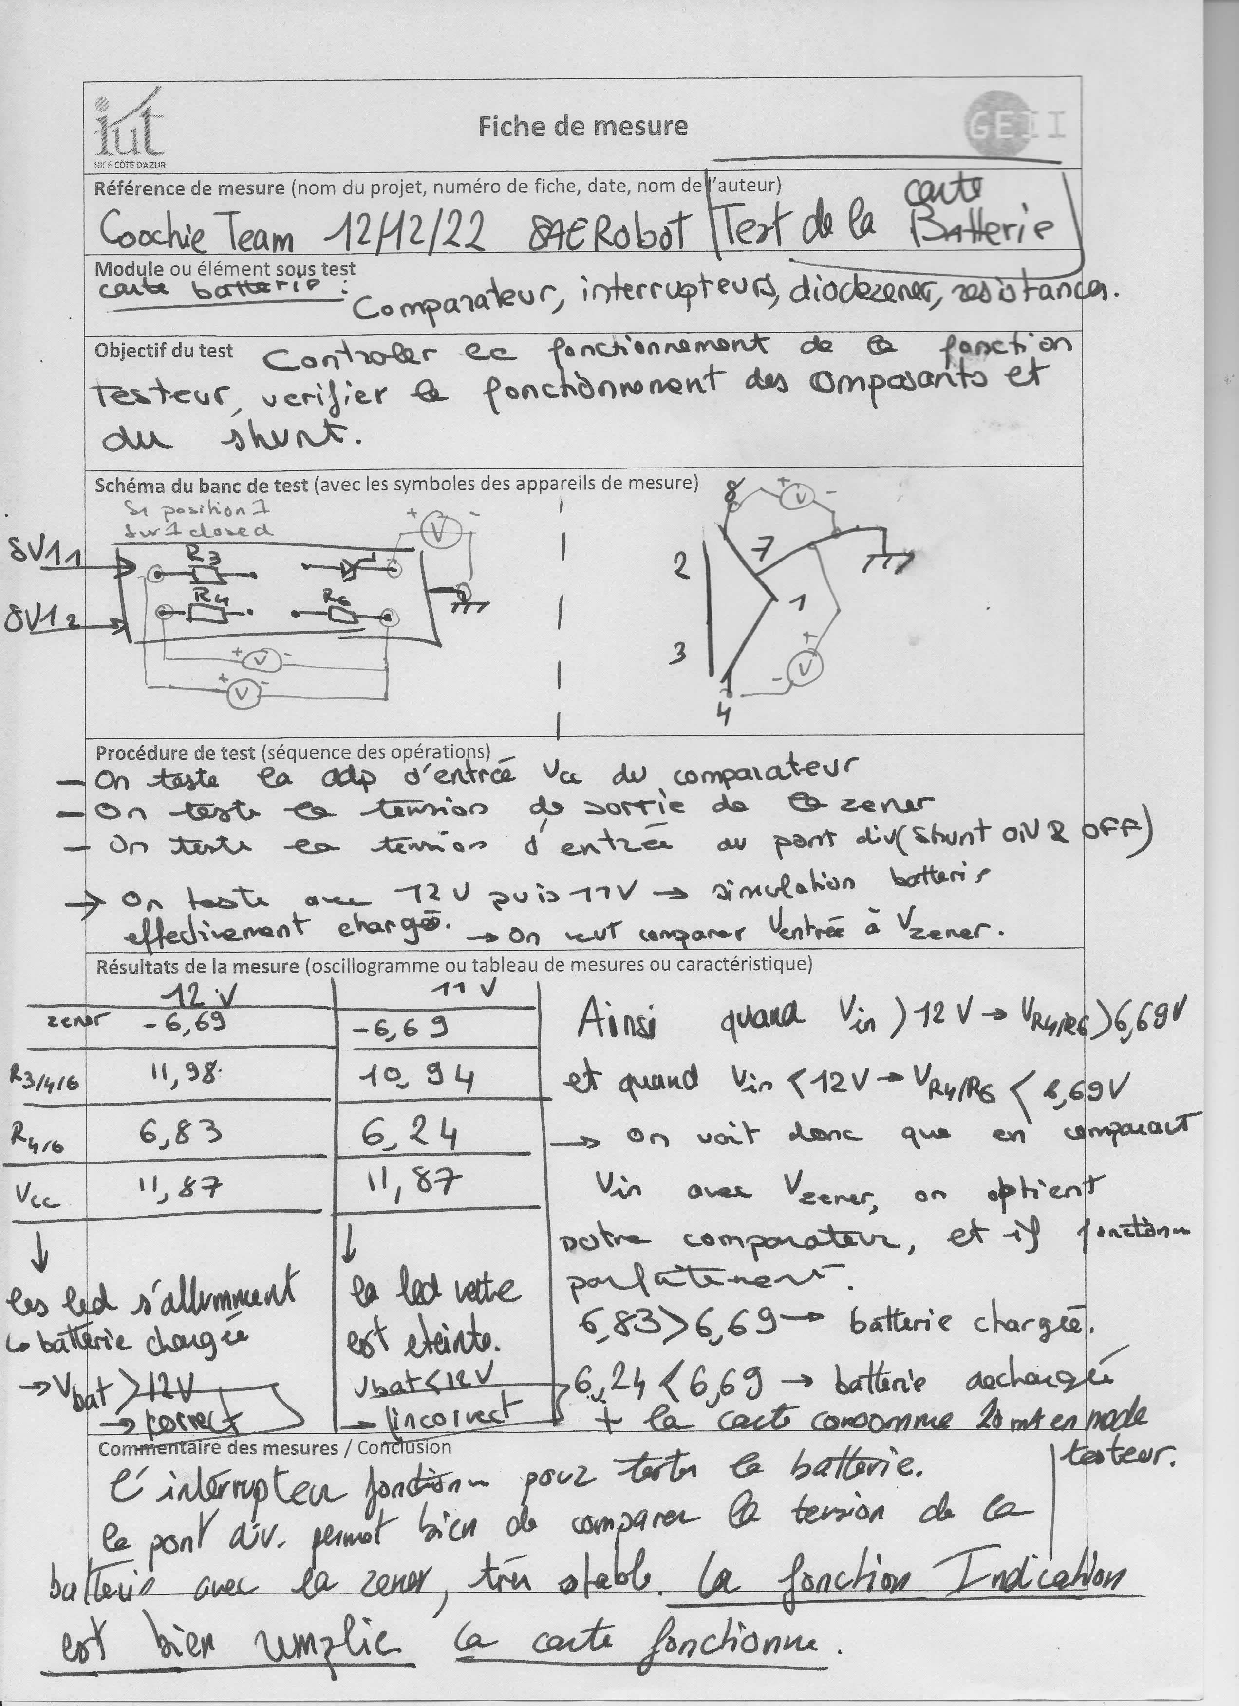
\includepdf[pages=-]{pdf/fichesmesure/degrade/Carte Batterie.pdf}

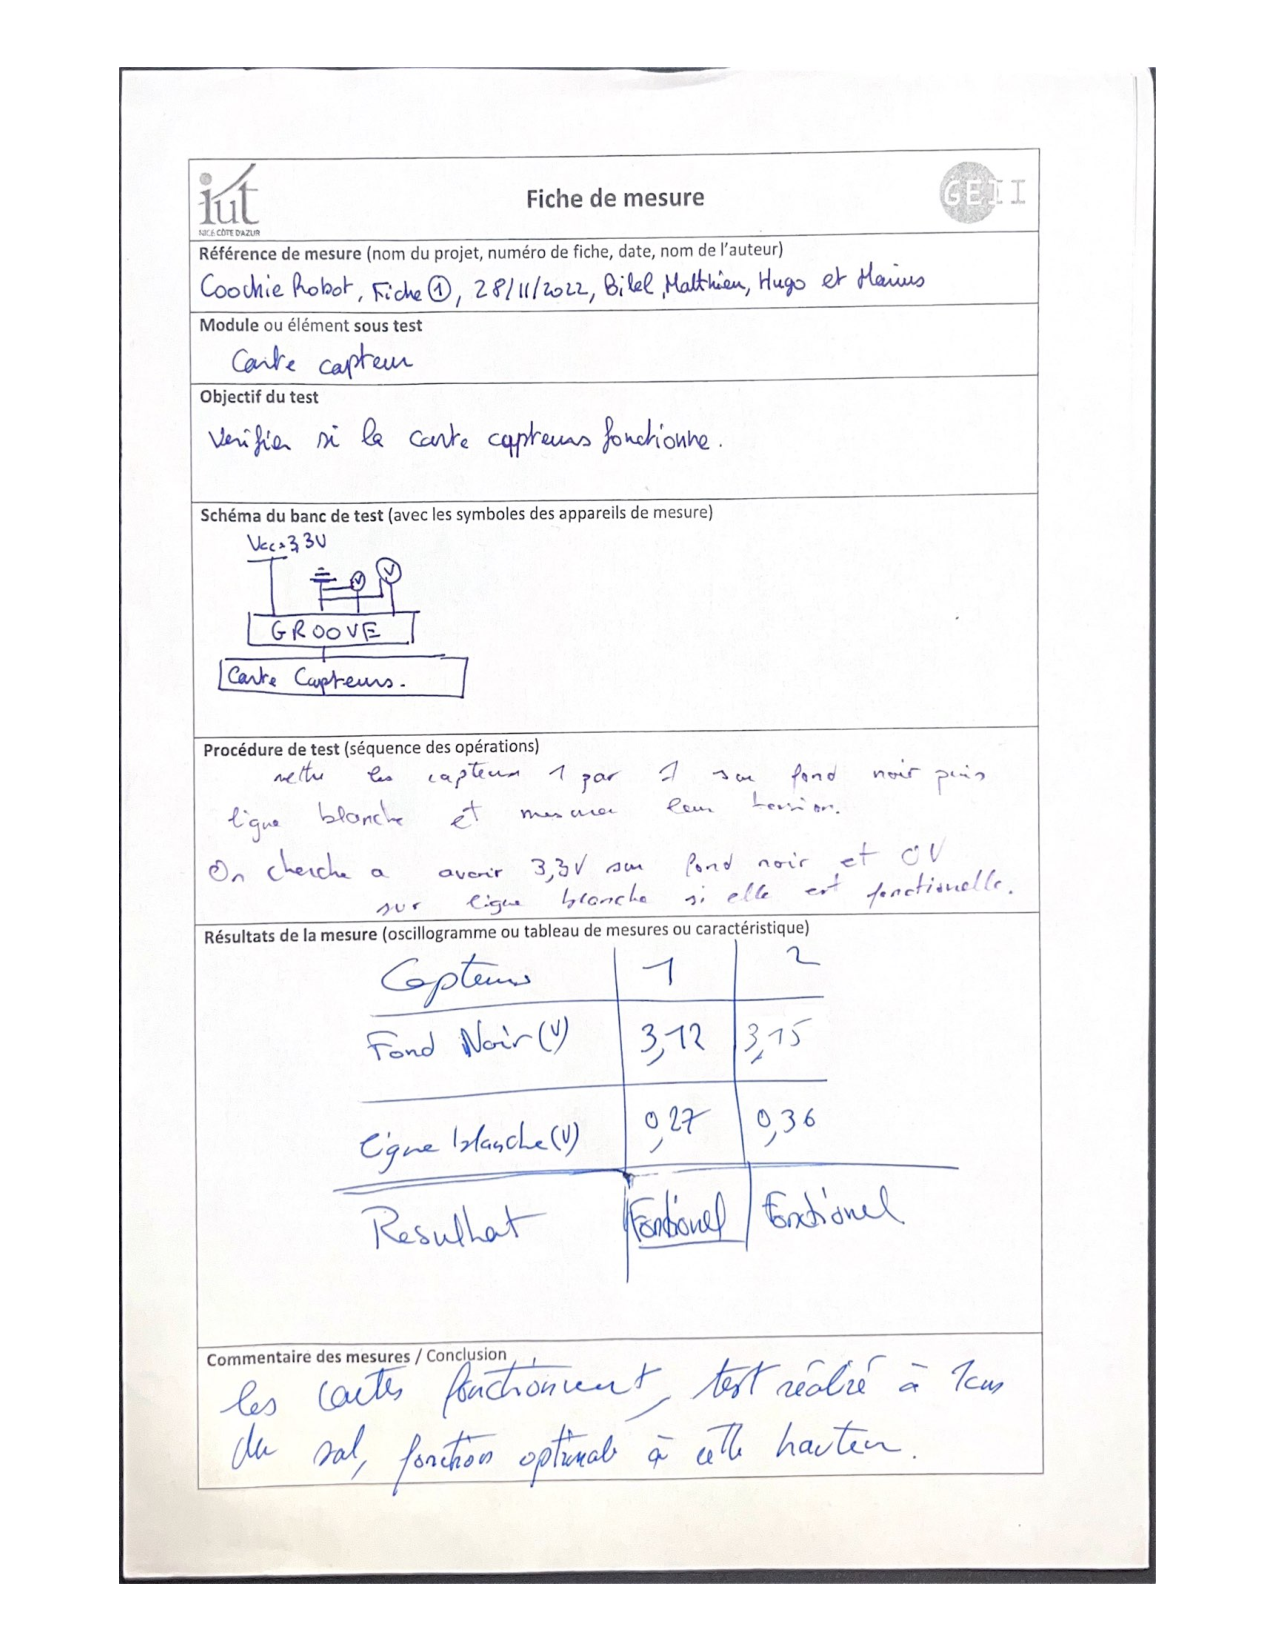
\includepdf[pages=-]{pdf/fichesmesure/degrade/Carte Capteurs.pdf}

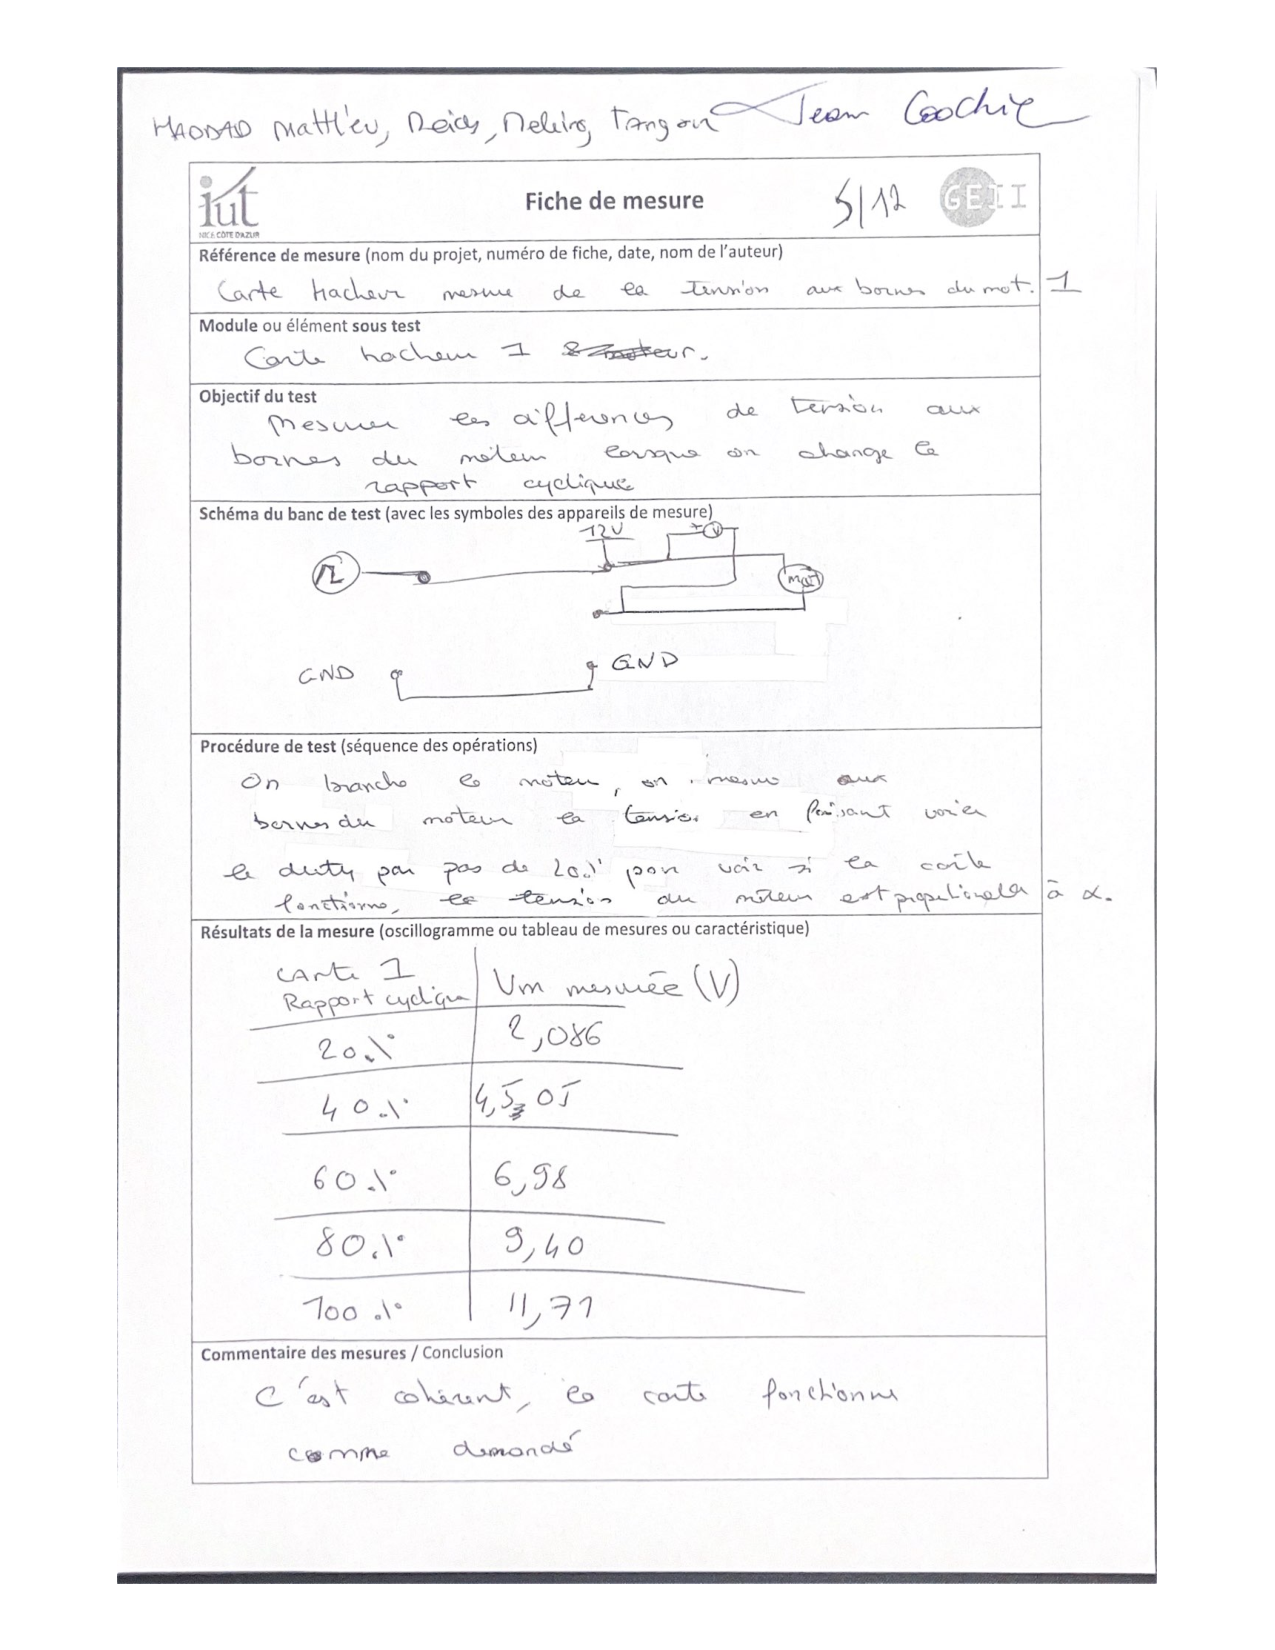
\includepdf[pages=-]{pdf/fichesmesure/degrade/Carte Hacheur.pdf}

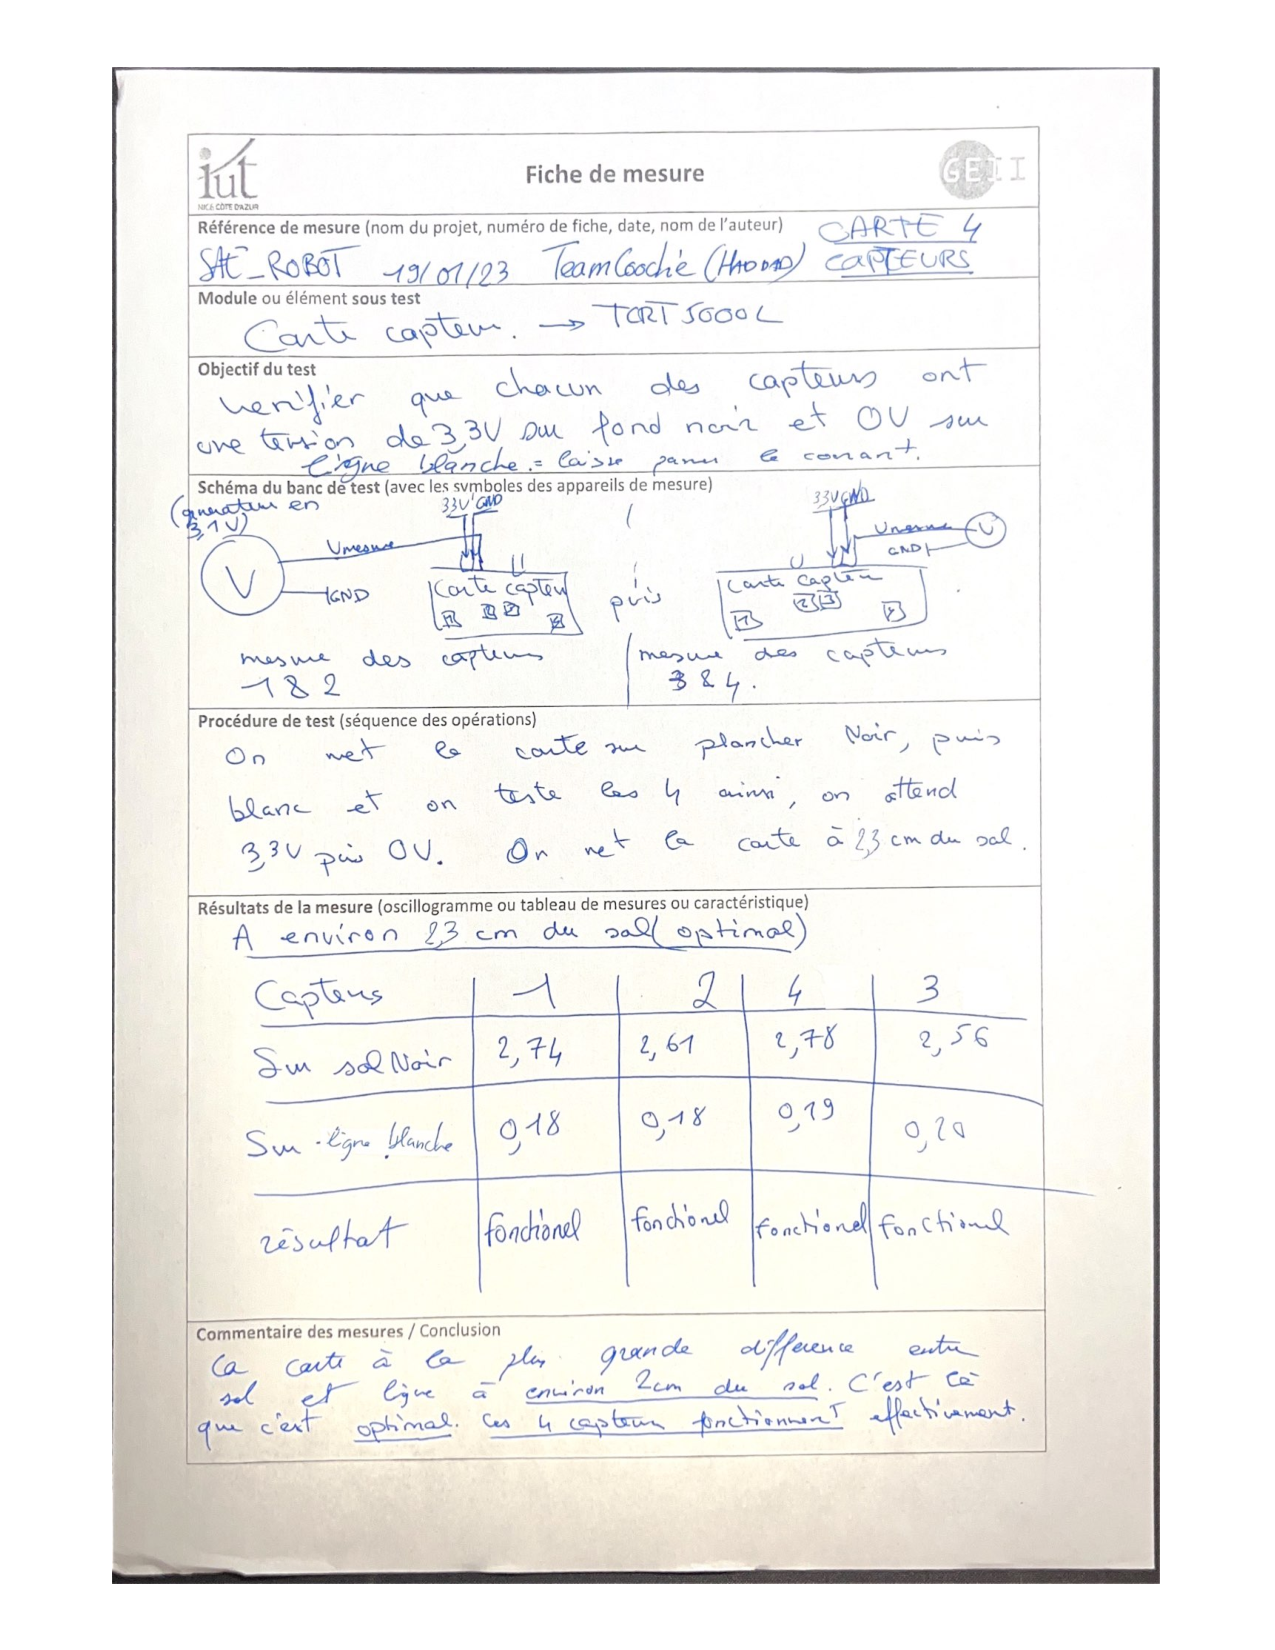
\includepdf[pages=-]{pdf/fichesmesure/designees/Carte Capteurs.pdf}

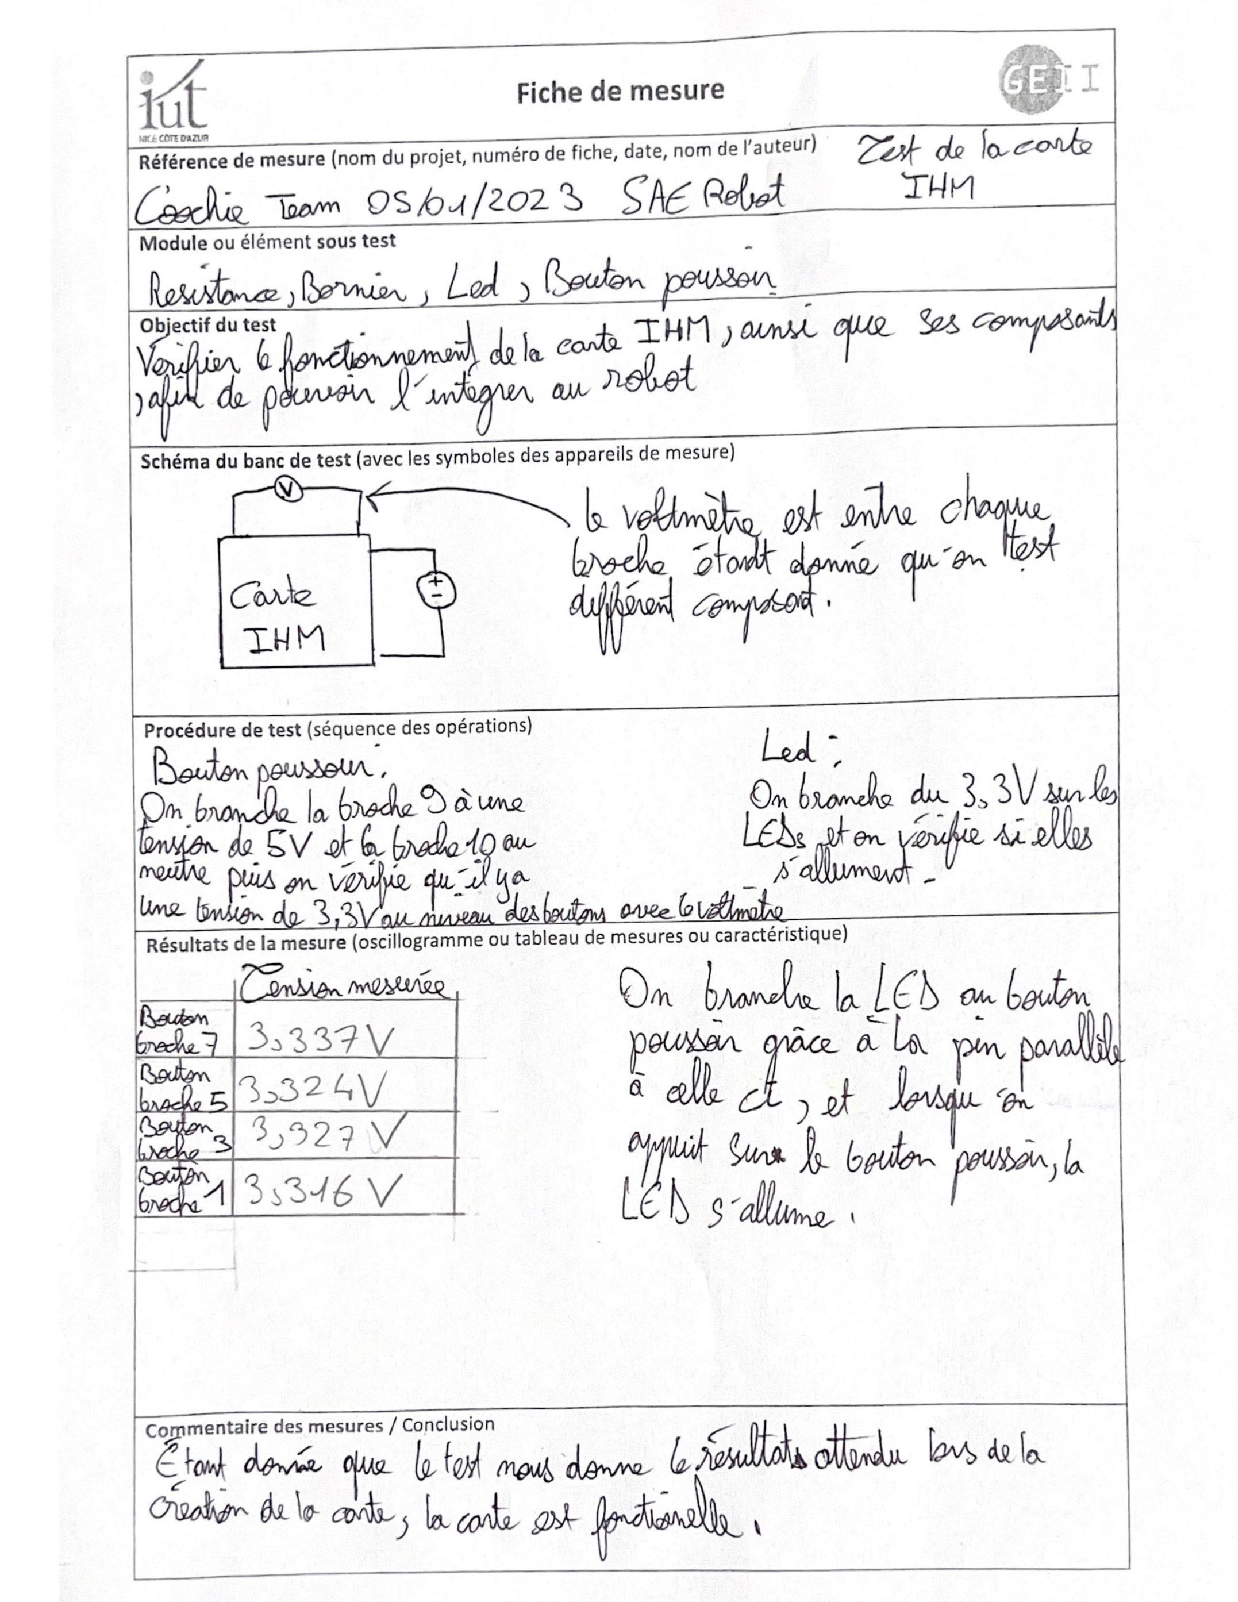
\includepdf[pages=-]{pdf/fichesmesure/designees/Carte IHM.pdf}

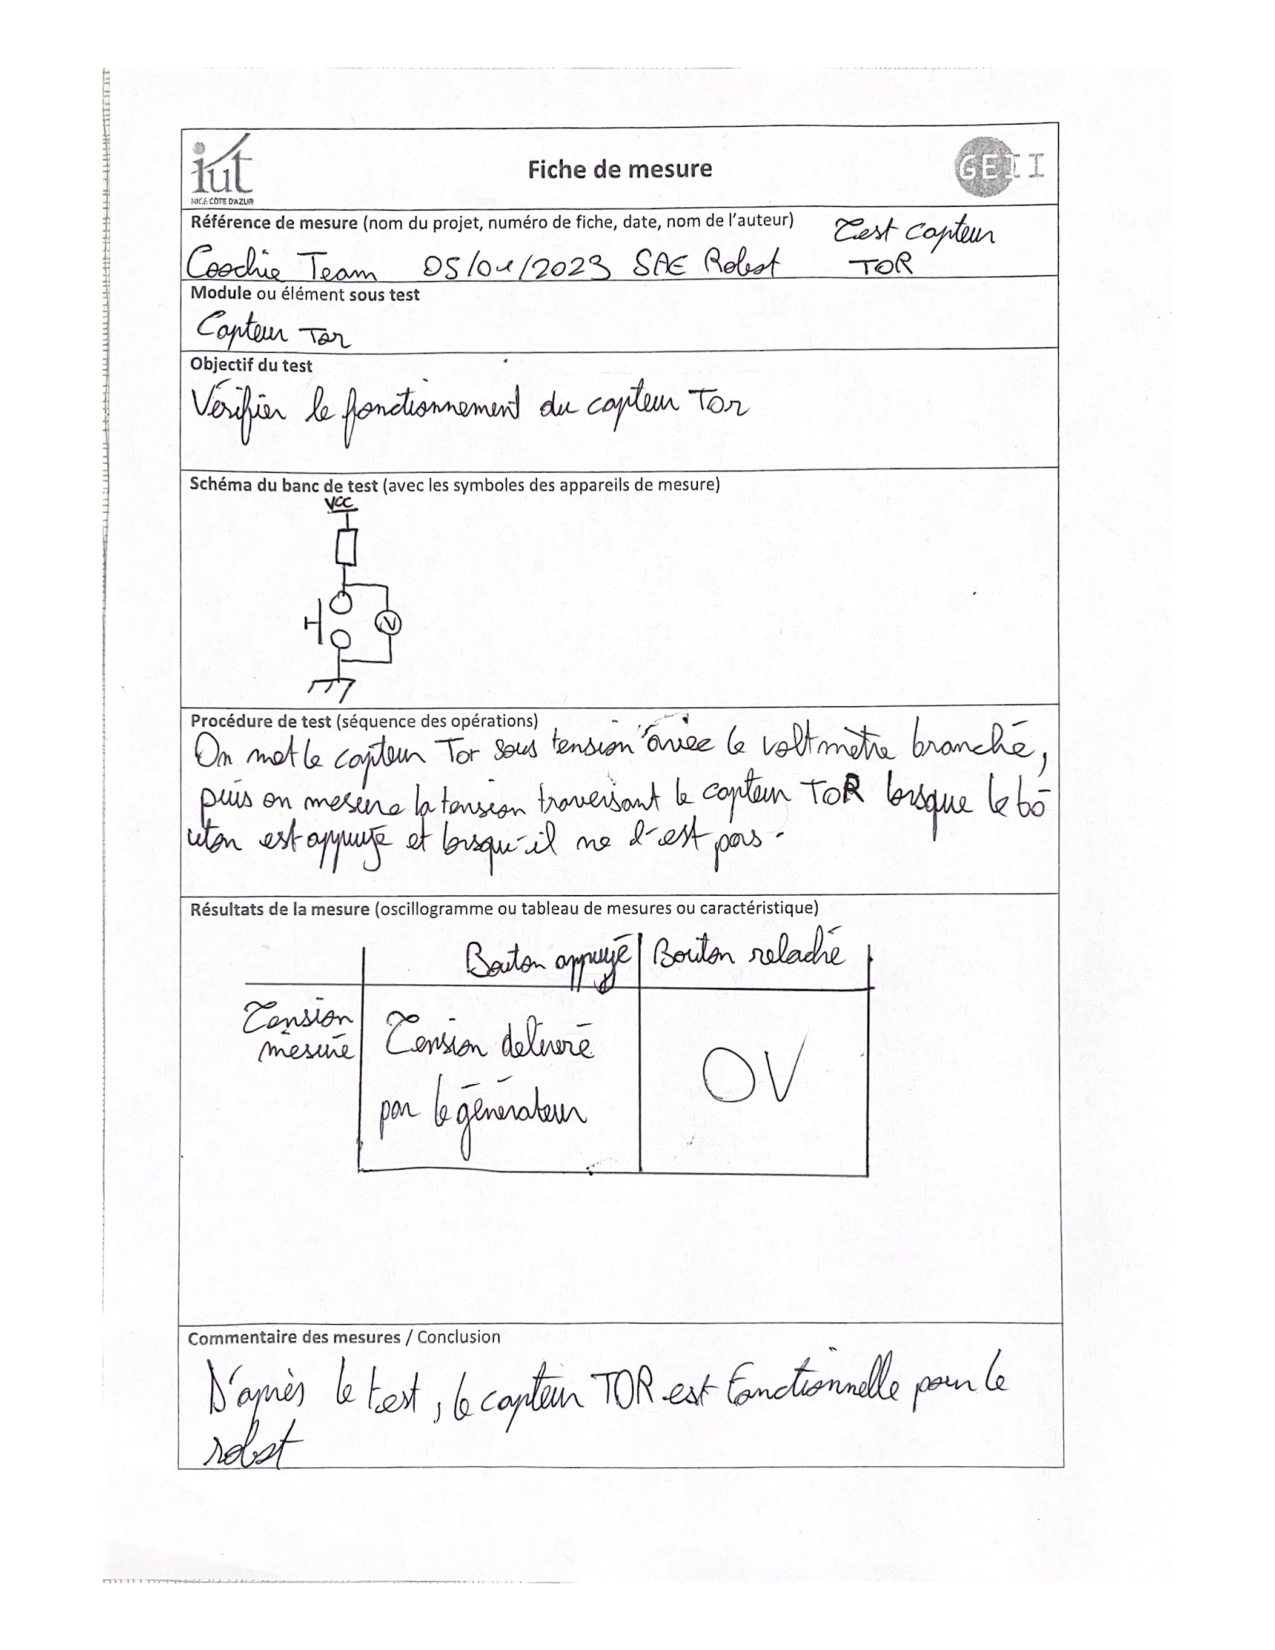
\includepdf[pages=-]{pdf/fichesmesure/designees/Capteur TOR.pdf}

\newpage

\thispagestyle{empty}
~
\vfill
\begin{center}

\large goofyBot - Coochie Team

\large I.U.T. Nice Côte d'Azur

\large 2023 | Conçu avec \LaTeX

\centering

\includegraphics[width=.3\linewidth]{img/logos/iut.png}
\end{center}